\chapter{核光滑方法}

% ============ 本章概述 ============

本章介绍一类\textbf{基于记忆（memory-based）}的回归与分类技术：在每个查询点 $x_0$ 处，仅使用 $x_0$ 附近的观测来拟合一个\textbf{局部简单模型}，并使得整体估计 $\hat{f}(X)$ 在 $\R^p$ 上光滑。这种局部化通过\textbf{核函数（kernel）} $K_\lambda(x_0, x)$ 实现——给 $x_i$ 分配一个随其到 $x_0$ 距离递减的权重，参数 $\lambda$ 控制邻域宽度。

\textbf{注意区分}：本章的「核」主要用于局部化（localization），与第5.8、12、14.5.4、18.5节中计算高维内积的「核方法」（kernel methods）不同，尽管在§6.7末尾会建立一些联系。

这类方法几乎不需要训练——所有工作都在评估时完成，唯一需要从训练数据确定的参数是 $\lambda$。

% ============ §6.1 一维核光滑器 ============
\section{一维核光滑器}

\subsection{从 $k$-最近邻平均到核加权平均}

在第2章中，$k$-最近邻平均
\begin{equation}\label{eq:knn_avg}
    \hat{f}(x_0) = \operatorname{Ave}(y_i \mid x_i \in N_k(x_0))
\end{equation}
被用作回归函数 $\E[Y \mid X = x_0]$ 的估计，其中 $N_k(x_0)$ 是距离 $x_0$ 最近的 $k$ 个点的集合。其思想是将条件期望的定义「松弛」——在目标点的邻域内做平均。

然而 $k$-NN 平均存在一个明显缺陷：$\hat{f}(x_0)$ 对 $x_0$ 是\textbf{不连续}的。当 $x_0$ 从左向右移动时，$k$-最近邻集合保持不变，直至某个右侧点比邻域中最远的左侧点更近——此时邻域成员发生替换，导致平均值跳跃。图6.1左面板展示了这种「颠簸」的绿色曲线。

\textbf{Nadaraya--Watson 核加权平均}通过给邻域内各点分配平滑递减的权重来解决此问题：
\begin{equation}\label{eq:nw_kernel}
    \hat{f}(x_0) = \frac{\sum_{i=1}^{N} K_\lambda(x_0, x_i) \, y_i}{\sum_{i=1}^{N} K_\lambda(x_0, x_i)}
\end{equation}
其中 $K_\lambda(x_0, x_i)$ 是核函数。使用 Epanechnikov 二次核时，拟合函数变为连续的且相当光滑（图6.1右面板）。

\begin{figure}[htbp]
    \centering
    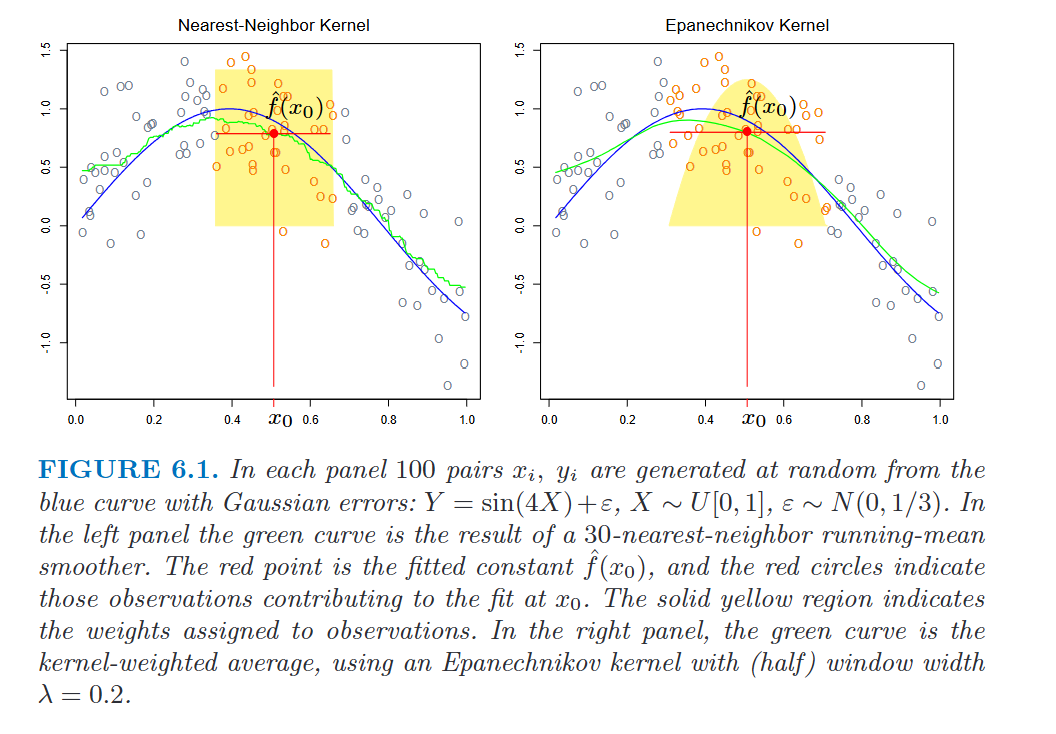
\includegraphics[width=0.95\textwidth]{Chapters/pic/ch_核光滑方法/figure_6_1.png}
    \caption{每面板中 100 对 $(x_i, y_i)$ 由蓝色曲线加高斯误差随机生成：$Y = \sin(4X) + \varepsilon$，$X \sim U[0,1]$，$\varepsilon \sim N(0, 1/3)$。\textbf{左面板}：绿色曲线是 30-最近邻滑动平均光滑器的结果。红点是拟合的常数 $\hat{f}(x_0)$，红色圆圈标示了参与 $x_0$ 处拟合的观测。黄色实心区域表示分配给各观测的权重。\textbf{右面板}：绿色曲线是核加权平均，使用 Epanechnikov 核，半窗宽 $\lambda = 0.2$。}
    \label{fig:6_1}
\end{figure}

\subsection{核函数的形式}

一般地，核函数可写为
\begin{equation}\label{eq:kernel_general}
    K_\lambda(x_0, x) = D\!\left(\frac{|x - x_0|}{h_\lambda(x_0)}\right)
\end{equation}
其中 $D(\cdot)$ 是核函数的具体形状，$h_\lambda(x_0)$ 是宽度函数（width function）。

\begin{itemize}
    \item \textbf{固定宽度（metric window）}：$h_\lambda(x_0) = \lambda$ 为常数，邻域宽度不随 $x_0$ 变化。
    \item \textbf{最近邻宽度}：$h_k(x_0) = |x_0 - x_{[k]}|$，其中 $x_{[k]}$ 是距离 $x_0$ 第 $k$ 近的点，邻域大小 $k$ 取代 $\lambda$ 作为参数。
\end{itemize}

\subsection{三种常用核}

在介绍具体核之前，先明确\textbf{紧支撑（compact support）}的数学含义：函数 $f$ 的支撑集定义为 $\operatorname{supp}(f) = \overline{\{x \mid f(x) \neq 0\}}$（即非零值集合的闭包）。若 $\operatorname{supp}(f)$ 是紧集（在 $\R^d$ 中等价于有界闭集），则称 $f$ 具有\textbf{紧支撑}。直观地说，紧支撑函数仅在有限范围内非零，范围之外恒为零——这对于结合最近邻窗宽使用的核是必要的。

\begin{itemize}
    \item \textbf{Epanechnikov 核}（紧支撑，边界处不可导）：
    \begin{equation}
        D(t) = \begin{cases}
            \frac{3}{4}(1 - t^2), & |t| \le 1 \\
            0, & \text{否则}
        \end{cases}
    \end{equation}

    \item \textbf{Tri-cube 核}（紧支撑，边界处有二阶连续导数，顶部更平坦）：
    \begin{equation}
        D(t) = \begin{cases}
            (1 - |t|^3)^3, & |t| \le 1 \\
            0, & \text{否则}
        \end{cases}
    \end{equation}

    \item \textbf{Gaussian 核}（非紧支撑，无穷可微）：
    \begin{equation}
        D(t) = \phi(t) = \frac{1}{\sqrt{2\pi}} e^{-t^2/2}
    \end{equation}
    标准差充当窗口宽度的角色。
\end{itemize}

\subsection{实践中的注意事项}

\begin{enumerate}
    \item \textbf{光滑参数 $\lambda$ 的选择}：$\lambda$ 大 → 方差低（平均更多观测）但偏差高（假设窗内函数为常数）。
    \item \textbf{固定宽度 vs 最近邻宽度的行为差异}：
    \begin{itemize}
        \item 固定宽度：偏差保持恒定，但方差与局部密度成反比；
        \item 最近邻宽度：方差保持恒定，绝对偏差与局部密度成反比。
    \end{itemize}
    \item \textbf{结（ties）的处理}：当 $x_i$ 存在重复值时，可以先对相同 $x$ 值处的 $y_i$ 做平均，并对合并后的观测赋予额外的权重 $w_i$。
    \item \textbf{观测权重} $w_i$：将 $w_i$ 乘以核权重后计算加权平均；在最近邻邻域中，使用权重总量 $k$（而非点数 $k$）来定义邻域。
    \item \textbf{边界问题}：固定宽度窗在边界处包含的点更少，而最近邻窗在边界处会变宽。
\end{enumerate}

% ============ §6.1.1 局部线性回归 ============
\section{局部线性回归}

\subsection{边界偏差问题}

尽管核加权平均已经比原始滑动平均光滑得多，但在\textbf{定义域边界附近}仍存在严重的偏差问题（图6.3左面板）。原因在于：边界处核是非对称的——邻域内大多数观测的均值高于目标点，因此即使加权后均值仍向上偏。

实际上，如果 $X$ 值不是等间距的，在定义域内部也可能存在类似偏差（通常程度较轻）。通过在局部拟合\textbf{直线}而非常数，可以精确到一阶地消除这种偏差。

\begin{figure}[htbp]
    \centering
    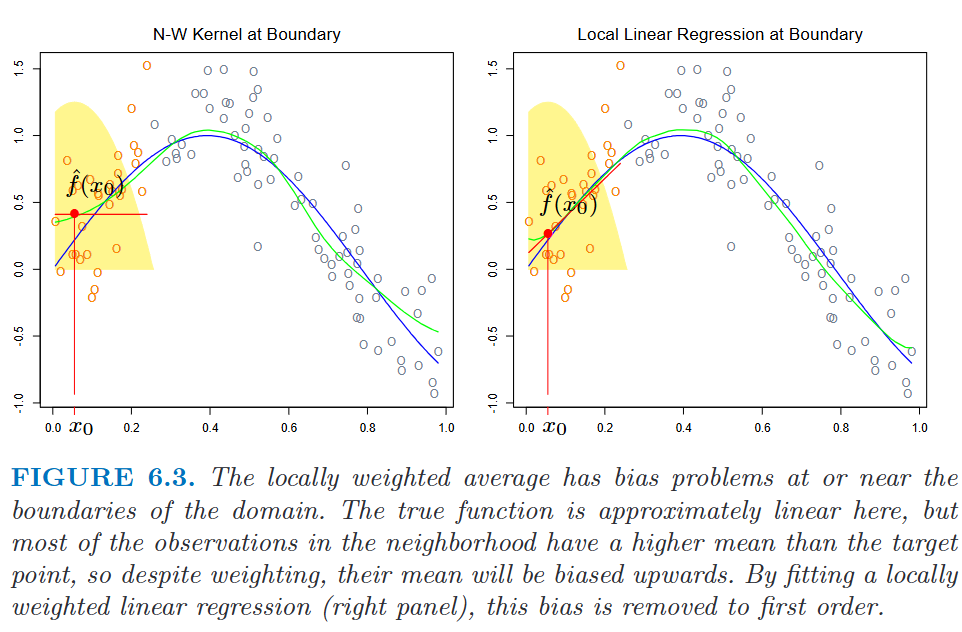
\includegraphics[width=0.95\textwidth]{Chapters/pic/ch_核光滑方法/figure_6_3.png}
    \caption{局部加权平均在定义域边界处或附近存在偏差问题。此处的真实函数近似线性，但邻域内大多数观测的均值高于目标点，因此即使加权后，其均值仍向上偏。通过在局部拟合加权线性回归（右面板），这一偏差被精确到一阶地消除。}
    \label{fig:6_3}
\end{figure}

\subsection{局部加权最小二乘}

在每个目标点 $x_0$ 处求解一个独立的加权最小二乘问题：
\begin{equation}\label{eq:local_linear}
    \min_{\alpha(x_0), \beta(x_0)} \sum_{i=1}^{N} K_\lambda(x_0, x_i) \bigl[y_i - \alpha(x_0) - \beta(x_0) x_i\bigr]^2
\end{equation}
估计值为 $\hat{f}(x_0) = \hat{\alpha}(x_0) + \hat{\beta}(x_0) x_0$。注意：虽然拟合了整个线性模型，但只在单点 $x_0$ 处使用。

\subsection{矩阵形式与等价核}

定义 $\mathbf{b}(x)^T = (1, x)$。设 $\mathbf{B}$ 为 $N \times 2$ 回归矩阵（第 $i$ 行为 $\mathbf{b}(x_i)^T$），$\mathbf{W}(x_0)$ 为 $N \times N$ 对角矩阵，第 $i$ 个对角元为 $K_\lambda(x_0, x_i)$。则
\begin{equation}\label{eq:local_linear_matrix}
    \hat{f}(x_0) = \mathbf{b}(x_0)^T \bigl(\mathbf{B}^T \mathbf{W}(x_0) \mathbf{B}\bigr)^{-1} \mathbf{B}^T \mathbf{W}(x_0) \mathbf{y}
    = \sum_{i=1}^{N} l_i(x_0) \, y_i
\end{equation}

权重 $l_i(x_0)$ 结合了核权重 $K_\lambda(x_0, \cdot)$ 和最小二乘操作，称为\textbf{等价核（equivalent kernel）}。$\hat{f}(x_0)$ 对 $y_i$ 是线性的（$l_i(x_0)$ 不依赖于 $y_i$）。

\subsection{自动核木工（Automatic Kernel Carpentry）}

历史上，Nadaraya--Watson 等局部平均核方法的偏差通过直接修改核函数来修正——这些修正基于渐近 MSE 理论，不仅实现繁琐，而且在有限样本下仅是近似的。局部线性回归能\textbf{自动}修改核以精确到一阶地校正偏差，这一现象被称为「自动核木工」。

考虑 $\E[\hat{f}(x_0)]$ 的展开（利用局部回归的线性和 $f$ 在 $x_0$ 处的 Taylor 展开）：
\begin{align}
    \E[\hat{f}(x_0)] &= \sum_{i=1}^{N} l_i(x_0) f(x_i) \nonumber \\
    &= f(x_0) \underbrace{\sum_{i=1}^{N} l_i(x_0)}_{=1}
       + f'(x_0) \underbrace{\sum_{i=1}^{N} (x_i - x_0) l_i(x_0)}_{=0}
       + \frac{f''(x_0)}{2} \sum_{i=1}^{N} (x_i - x_0)^2 l_i(x_0) + R \label{eq:bias_expansion}
\end{align}
其中余项 $R$ 涉及 $f$ 的三阶及以上导数，在适当光滑性假设下通常很小。对于局部线性回归，可证 $\sum l_i(x_0) = 1$ 且 $\sum (x_i - x_0) l_i(x_0) = 0$（习题6.2），因此偏差 $\E[\hat{f}(x_0)] - f(x_0)$ 仅依赖于 $f$ 展开中的二阶及更高阶项——一阶偏差被完全消除。

\medskip
\textbf{Q：自动核木工（Automatic Kernel Carpentry）到底在说什么？}

可以从「等价核」的角度来理解。Nadaraya--Watson 核加权平均本质上等价于用一个\textbf{给定的}核 $D(\cdot)$ 做局部常数拟合。这个固定形状的核在边界处不对称，导致一阶偏差。历史上人们试图通过手工设计「高阶核」（higher-order kernels）来修正——让核函数满足特定的矩条件（如 $\int t K(t) dt = 0$），从而消除低阶偏差。但这需要针对不同情况手工调整核的形状和参数，实现繁琐，且只在渐近意义下精确。

局部线性回归的巧妙之处在于：它不直接修改 $K_\lambda$，而是通过最小二乘的代数结构\textbf{自动生成了正确的等价核} $l_i(x_0)$。从式(\ref{eq:bias_expansion})可以看到，只要等价权重满足 $\sum l_i = 1$ 和 $\sum (x_i - x_0)l_i = 0$，一阶偏差就自动消失——而局部线性回归的最小二乘解恰好保证这两个条件成立，无需任何手工调整。换句话说，与其自己费劲「雕琢」核函数的形状来消偏差，不如让最小二乘帮你自动「打磨」出正确的权重——这就是「自动核木工」（automatic kernel carpentry）这个比喻的含义。

\medskip
\textbf{Q：在实践中是怎么利用这个方法的？}

实践者几乎不需要关心核木工的细节——它对你完全透明。你只需要在使用局部回归软件时选择\textbf{局部线性}（$d=1$）而非局部常数（$d=0$），偏差校正就自动生效。具体来说：

\begin{itemize}
    \item 在 R 的 \texttt{loess()} 或 \texttt{locfit} 中，设置 \texttt{degree=1}（通常这就是默认值）；
    \item 在 Python 的 \texttt{statsmodels.nonparametric.KernelReg} 中，选择 \texttt{reg\_type='ll'}（local linear）。
\end{itemize}

你实际要做的决策只有两个：(1) 选什么核（tri-cube 是常用默认，紧支撑且边界光滑）；(2) 选多大窗宽 $\lambda$（通过交叉验证确定）。选好之后直接拟合，边界处的偏差自动被一阶校正——不需要你手工设计高阶核，也不需要区分边界和内部做不同处理。这就是自动核木工给实践者带来的便利：用局部线性替代局部常数几乎只有收益（以微小的方差增加换取大幅的边界偏差降低），所以局部线性已经成为了局部多项式回归的事实标准。

% ============ §6.1.2 局部多项式回归 ============
\section{局部多项式回归}

\subsection{$d$ 阶局部多项式拟合}

将局部拟合从线性推广到任意 $d$ 次多项式：
\begin{equation}\label{eq:local_poly}
    \min_{\alpha(x_0), \beta_j(x_0)} \sum_{i=1}^{N} K_\lambda(x_0, x_i) \left[y_i - \alpha(x_0) - \sum_{j=1}^{d} \beta_j(x_0) x_i^j\right]^2
\end{equation}
估计值为 $\hat{f}(x_0) = \hat{\alpha}(x_0) + \sum_{j=1}^{d} \hat{\beta}_j(x_0) x_0^j$。类似式(\ref{eq:bias_expansion})的展开表明，偏差仅包含 $d+1$ 阶及以上的分量（习题6.2）。

\subsection{削峰填谷效应}

局部线性拟合在真实函数有曲率的区域存在偏差——这一现象称为「\textbf{削峰填谷（trimming the hills and filling the valleys）}」：线性拟合倾向于低估峰值、高估谷底。局部二次回归通常能够校正这种曲率偏差（图6.5）。

\begin{figure}[htbp]
    \centering
    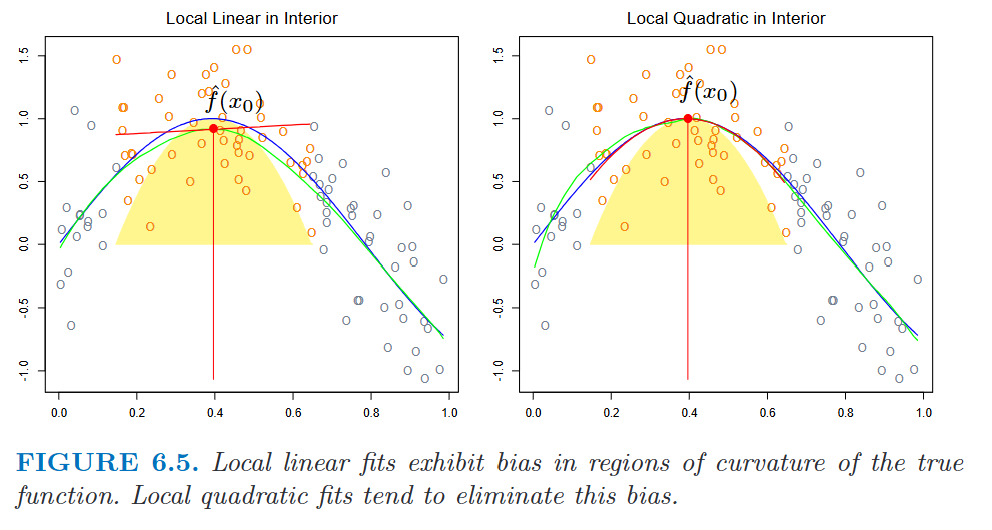
\includegraphics[width=0.95\textwidth]{Chapters/pic/ch_核光滑方法/figure_6_5.png}
    \caption{局部线性拟合在真实函数曲率区域表现出偏差。局部二次拟合倾向于消除此偏差。左面板中红色曲线（局部线性）在曲率处偏离绿色真实曲线，右面板中局部二次拟合更好地追踪了曲率。}
    \label{fig:6_5}
\end{figure}

\subsection{偏差--方差权衡}

偏差降低的代价是方差增大。假设模型 $y_i = f(x_i) + \varepsilon_i$，$\varepsilon_i \sim \text{i.i.d.}(0, \sigma^2)$，则
\begin{equation}\label{eq:local_var}
    \Var(\hat{f}(x_0)) = \sigma^2 \, \|\mathbf{l}(x_0)\|^2
\end{equation}
其中 $\mathbf{l}(x_0)$ 是等价核权重向量。可证 $\|\mathbf{l}(x_0)\|^2$ 随 $d$ 增加而增大（习题6.3），因此存在偏差--方差权衡。

图6.6展示了局部常数、线性、二次回归的方差函数曲线。

\subsection{奇数阶 vs 偶数阶：实践建议}

\begin{itemize}
    \item 局部线性拟合（$d=1$）能以\textbf{适度的方差代价}在边界处大幅降低偏差；局部二次拟合（$d=2$）在边界处对偏差改善不大，但方差增加很多。
    \item 局部二次拟合最有助于减少\textbf{定义域内部的曲率偏差}。
    \item 渐近分析表明，\textbf{奇数阶局部多项式优于偶数阶}——这主要是因为渐近 MSE 由边界效应主导。
\end{itemize}

通常由应用场景决定拟合阶数：若关注外推，则边界更重要，局部线性拟合更可靠。不推荐在不同区域使用不同阶数的策略。

% ============ §6.2 核宽度的选择 ============
\section{核宽度的选择}

\subsection{$\lambda$ 在不同核中的含义}

\begin{itemize}
    \item Epanechnikov 或 tri-cube 核（固定宽度）：$\lambda$ 是支撑区域的半径。
    \item Gaussian 核：$\lambda$ 是标准差。
    \item $k$-最近邻：$\lambda$ 是近邻数 $k$，通常表示为总训练样本的比例（span）$k/N$。
\end{itemize}

\subsection{偏差--方差权衡与窗宽}

改变平均窗宽时存在自然的偏差--方差权衡，以局部平均为例最为直观：

\begin{itemize}
    \item \textbf{窄窗}：$\hat{f}(x_0)$ 仅对 $x_0$ 附近少数 $y_i$ 做平均，方差较大（接近单个 $y_i$ 的方差）；偏差较小——因为每个 $\E(y_i) = f(x_i)$ 都接近 $f(x_0)$。
    \item \textbf{宽窗}：$\hat{f}(x_0)$ 的方差因平均效应而较小；偏差较大——使用了远离 $x_0$ 的 $x_i$，无法保证 $f(x_i)$ 接近 $f(x_0)$。
\end{itemize}

对局部回归估计（如局部线性）类似：窗宽趋于零时，估计趋近于\textbf{插值训练数据的分段线性函数}；窗宽趋于无穷时，拟合趋近于\textbf{全局线性最小二乘拟合}。

\subsection{线性估计量与光滑矩阵}

局部回归光滑器是\textbf{线性估计量}：$\hat{\mathbf{f}} = \mathbf{S}_\lambda \mathbf{y}$。光滑矩阵 $\mathbf{S}_\lambda$ 由等价核构建，其第 $ij$ 个元素为 $\{\mathbf{S}_\lambda\}_{ij} = l_i(x_j)$。

\medskip
\textbf{为什么称 $\mathbf{S}_\lambda$ 为「光滑」算子？核 $K_\lambda$ 去哪了？}

核 $K_\lambda$ 并没有消失——它被「吸收」进了 $\mathbf{S}_\lambda$。从局部线性回归的矩阵形式
\[
\hat{f}(x_0) = \mathbf{b}(x_0)^T (\mathbf{B}^T \mathbf{W}(x_0) \mathbf{B})^{-1} \mathbf{B}^T \mathbf{W}(x_0) \mathbf{y}
\]
可以看到，核权重通过 $\mathbf{W}(x_0)$（对角元为 $K_\lambda(x_0, x_i)$）进入计算，再经过最小二乘的代数运算，最终凝练为等价核权重 $l_i(x_0)$。$\mathbf{S}_\lambda$ 的第 $j$ 列正是对所有 $x_j$ 的等价核在这些训练点上的取值排列。

称 $\mathbf{S}_\lambda$ 为「光滑矩阵」（smoother matrix）是因为：(1) 从效果上看，$\hat{\mathbf{f}} = \mathbf{S}_\lambda \mathbf{y}$ 确实在\textbf{光滑}原始响应 $y_i$——把带噪声的点云变成一条平滑曲线；(2) 这一写法是\textbf{统一的框架}——不仅核光滑器，光滑样条、回归样条等所有线性光滑方法都可以写成 $\hat{\mathbf{f}} = \mathbf{S}_\lambda \mathbf{y}$ 的形式，便于用统一语言讨论自由度、交叉验证等概念。核的作用在构造 $\mathbf{S}_\lambda$ 的阶段已经完成，后续分析直接使用 $\mathbf{S}_\lambda$ 即可。

\medskip
\textbf{交叉验证（CV）在局部回归中的具体做法}

因为 $\hat{\mathbf{f}} = \mathbf{S}_\lambda \mathbf{y}$ 是\textbf{线性}估计量，交叉验证有非常简洁的计算公式，无需反复重新拟合。

\textbf{留一交叉验证（LOOCV）。} 记 $\hat{f}^{(-i)}(x_i)$ 为去掉第 $i$ 个观测后模型在 $x_i$ 处的预测。LOOCV 准则为
\[
\text{CV}(\lambda) = \frac{1}{N} \sum_{i=1}^{N} \bigl(y_i - \hat{f}^{(-i)}(x_i)\bigr)^2
\]
由于 $\hat{f}^{(-i)}(x_i)$ 可写为 $\hat{f}^{(-i)}(x_i) = \sum_{j \neq i} \frac{S_{ij}}{1 - S_{ii}} \, y_j$（习题6.7），经过代数推导得到捷径公式：
\begin{equation}\label{eq:loocv_shortcut}
    \text{CV}(\lambda) = \frac{1}{N} \sum_{i=1}^{N} \left[ \frac{y_i - \hat{f}(x_i)}{1 - S_{ii}} \right]^2
\end{equation}
这意味着只需\textbf{拟合一次}全模型得到 $\hat{\mathbf{f}}$ 和 $S_{ii}$（$\mathbf{S}_\lambda$ 的对角元），即可计算 LOOCV——极大地节省了计算量。

\textbf{广义交叉验证（GCV）。} GCV 将 $S_{ii}$ 替换为其平均值 $\frac{1}{N} \sum_i S_{ii} = \frac{\tr(\mathbf{S}_\lambda)}{N} = \frac{\text{df}_\lambda}{N}$：
\begin{equation}\label{eq:gcv}
    \text{GCV}(\lambda) = \frac{1}{N} \sum_{i=1}^{N} \left[ \frac{y_i - \hat{f}(x_i)}{1 - \tr(\mathbf{S}_\lambda)/N} \right]^2
    = \frac{\text{RSS}/N}{(1 - \text{df}_\lambda / N)^2}
\end{equation}
GCV 的优势在于：(1) 不需要逐个计算 $S_{ii}$，只需 $\tr(\mathbf{S}_\lambda)$；(2) 具有某些不变性（如在正交变换下不变）；(3) 在许多情况下与 LOOCV 表现接近。

\textbf{$k$-折交叉验证。} 将数据随机分为 $k$ 个大小相近的折，每次留一折作为验证集，其余 $k-1$ 折训练。计算量比 LOOCV 小（只需 $k$ 次拟合），但无法使用上述捷径公式。实践中 $k=5$ 或 $k=10$ 较为常用。

选择 $\lambda$ 时，在 $\lambda$ 的候选网格上计算 CV/GCV 得分，选择使得分最小的 $\lambda$。这一过程对局部平均和局部回归均适用。

\subsection{有效自由度}

\textbf{有效自由度}定义为 $\text{df}_\lambda = \tr(\mathbf{S}_\lambda)$，可用于校准光滑量。

\begin{figure}[htbp]
    \centering
    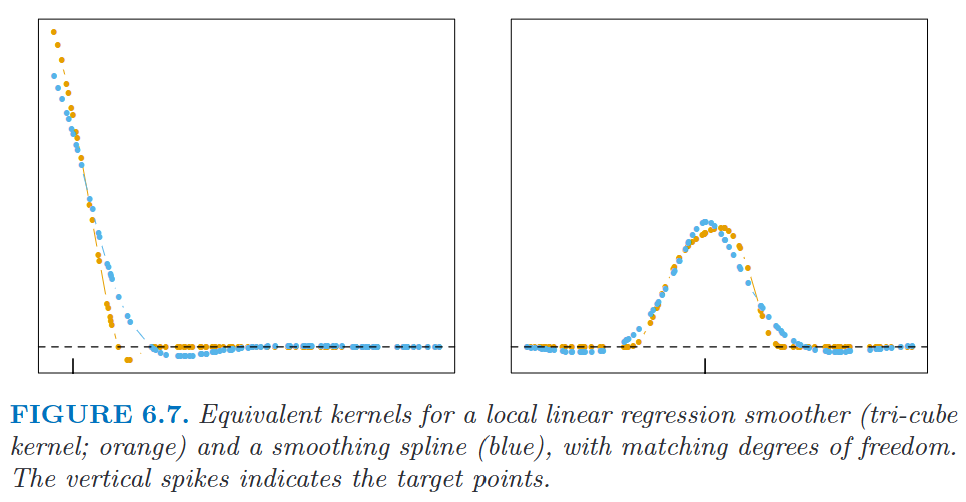
\includegraphics[width=0.9\textwidth]{Chapters/pic/ch_核光滑方法/figure_6_7.png}
    \caption{局部线性回归光滑器（tri-cube 核，橙色）与光滑样条（蓝色）的等价核，两者具有匹配的自由度。竖直尖刺标示目标点。局部回归光滑器的 span 为 40\%，对应 $\text{df} = \tr(\mathbf{S}_\lambda) = 5.86$；光滑样条被校准到相同 df，两者的等价核定性上高度相似。}
    \label{fig:6_7}
\end{figure}

% ============ §6.3 IR^p 中的局部回归 ============
\section{$\R^p$ 中的局部回归}

核光滑和局部回归可以非常自然地推广到二维及以上。Nadaraya--Watson 核光滑器使用 $p$ 维核提供的权重在局部拟合常数；局部线性回归则通过加权最小二乘在 $X$ 空间中局部拟合超平面，实现简单且边界性能优于局部常数拟合。

\subsection{多项式向量与径向核}

设 $\mathbf{b}(X)$ 为 $X$ 中最大次数为 $d$ 的多项式项向量。例如：
\begin{itemize}
    \item $d=1,\; p=2$：$\mathbf{b}(X) = (1, X_1, X_2)$；
    \item $d=2,\; p=2$：$\mathbf{b}(X) = (1, X_1, X_2, X_1^2, X_2^2, X_1 X_2)$；
    \item $d=0$：$\mathbf{b}(X) = 1$（退化为局部常数）。
\end{itemize}

在每个 $x_0 \in \R^p$ 处求解
\begin{equation}\label{eq:local_poly_p}
    \min_{\beta(x_0)} \sum_{i=1}^{N} K_\lambda(x_0, x_i) \bigl(y_i - \mathbf{b}(x_i)^T \beta(x_0)\bigr)^2
\end{equation}
得到拟合 $\hat{f}(x_0) = \mathbf{b}(x_0)^T \hat{\beta}(x_0)$。

核通常采用\textbf{径向函数}，如径向 Epanechnikov 或 tri-cube 核：
\begin{equation}\label{eq:radial_kernel}
    K_\lambda(x_0, x) = D\!\left(\frac{\|x - x_0\|}{\lambda}\right)
\end{equation}
其中 $\|\cdot\|$ 为欧氏距离。由于欧氏距离依赖于各坐标的单位，最合理的做法是先在平滑前将每个预测变量\textbf{标准化}（如标准化到单位标准差）。

\subsection{高维中的边界问题与维数灾难}

边界效应在一维平滑中是一个问题，但在二维或更高维中更为严重——边界上点的比例更大。事实上，\textbf{维数灾难}的一个表现就是：随着维数增长，靠近边界的点的比例趋近于 1。直接修改核以适应二维边界非常繁琐（尤其对于不规则边界），而局部多项式回归能在任意维度下无缝地完成所需阶数的边界校正。

然而，局部回归在维数远高于 2 或 3 时变得不太有用。第2章已详细讨论过维数问题：随着维数增加，不可能同时保持局部性（低偏差）和邻域内有足够的样本量（低方差），除非总样本量随 $p$ 指数增长。此外，$\hat{f}(X)$ 的可视化在高维也变得困难——而这往往是平滑的主要目标之一。从数据分析的角度看，条件图（conditional plots）远比散点云和线框图更有用（图6.9的 trellis 展示）。

% ============ §6.4 IR^p 中的结构化局部回归模型 ============
\section{$\R^p$ 中的结构化局部回归模型}

当维数与样本量之比不利时，局部回归的帮助有限——除非我们愿意对模型施加一些结构性假设。

\subsection{结构化核}

一种思路是修改核函数。默认的球形核（式\ref{eq:radial_kernel}）对各坐标赋予等权重，因此自然的默认策略是将每个变量标准化到单位标准差。更一般的方法是用一个半正定矩阵 $\mathbf{A}$ 对不同坐标加权：
\begin{equation}\label{eq:structured_kernel}
    K_{\lambda, \mathbf{A}}(x_0, x) = D\!\left(\frac{(x - x_0)^T \mathbf{A} (x - x_0)}{\lambda}\right)
\end{equation}
通过对 $\mathbf{A}$ 施加适当的限制，可以降权或忽略某些坐标或方向。例如，若 $\mathbf{A}$ 为对角阵，则可以增大或减小单个预测变量 $X_j$ 的影响。当预测变量多且高度相关时（如来自数字化模拟信号或图像），可利用预测变量的协方差函数来定制度量 $\mathbf{A}$，使对高频对比的关注减少。也有方法尝试学习多维核的参数（如第11章中的投影寻踪回归）。

\subsection{结构化回归函数}

我们试图在 $\R^p$ 中拟合 $f(X_1, X_2, \ldots, X_p)$，其中可能存在各种交互。自然的思路是考虑\textbf{方差分析（ANOVA）分解}：
\begin{equation}\label{eq:anova_decomp}
    f(X_1, \ldots, X_p) = \alpha + \sum_j g_j(X_j) + \sum_{k<\ell} g_{k\ell}(X_k, X_\ell) + \cdots
\end{equation}
然后通过去掉某些高阶项来引入结构。

\textbf{可加模型}仅保留主效应项：$f(X) = \alpha + \sum_{j=1}^{p} g_j(X_j)$。二阶模型最多包含二阶交互项，以此类推。第9章描述了用于拟合此类低阶交互模型的\textbf{迭代 backfitting 算法}。以可加模型为例：若假设除第 $k$ 项外所有项已知，则可通过 $Y - \sum_{j \neq k} g_j(X_j)$ 对 $X_k$ 的局部回归来估计 $g_k$；轮流对每个函数重复此操作直至收敛。关键细节是：在任何阶段都只需一维局部回归。

\subsection{变系数模型}

结构化模型的一个重要特例是\textbf{变系数模型（varying coefficient models）}。将 $p$ 个预测变量划分为集合 $(X_1, \ldots, X_q)$（$q < p$）和 $Z$，假设条件线性模型：
\begin{equation}\label{eq:varying_coef}
    f(X) = \alpha(Z) + \beta_1(Z) X_1 + \cdots + \beta_q(Z) X_q
\end{equation}
对给定的 $Z$，这是线性模型，但每个系数可随 $Z$ 变化。自然地通过局部加权最小二乘拟合：
\begin{equation}\label{eq:varying_coef_fit}
    \min_{\alpha(z_0), \beta(z_0)} \sum_{i=1}^{N} K_\lambda(z_0, z_i) \bigl(y_i - \alpha(z_0) - x_{1i}\beta_1(z_0) - \cdots - x_{qi}\beta_q(z_0)\bigr)^2
\end{equation}

图6.10--6.11 以人体主动脉数据为例：将主动脉直径建模为年龄的线性函数，但允许系数随性别和沿主动脉的深度变化。

% ============ §6.5 局部似然与其他模型 ============
\section{局部似然与其他模型}

局部回归和变系数模型的概念非常广泛：只要拟合方法支持观测权重，任何参数模型都可以「局部化」。

\subsection{局部似然}

设每个观测 $y_i$ 关联一个参数 $\theta_i = \theta(x_i) = x_i^T \beta$，基于对数似然 $l(\beta) = \sum_i l(y_i, x_i^T \beta)$ 对 $\beta$ 做推断。通过使用 $x_0$ 处的局部似然，可以对 $\theta(x_0) = x_0^T \beta(x_0)$ 做更灵活的推断：
\begin{equation}\label{eq:local_likelihood}
    l(\beta(x_0)) = \sum_{i=1}^{N} K_\lambda(x_0, x_i) \, l\bigl(y_i, x_i^T \beta(x_0)\bigr)
\end{equation}
许多似然模型——特别是广义线性模型家族（包括 logistic 和对数线性模型）——以线性方式引入协变量。局部似然允许从全局线性模型松弛到局部线性模型。

进一步，定义 $\theta$ 的变量和用于定义局部似然的变量可以不同：
\begin{equation}
    l(\theta(z_0)) = \sum_{i=1}^{N} K_\lambda(z_0, z_i) \, l\bigl(y_i, \eta(x_i, \theta(z_0))\bigr)
\end{equation}
例如 $\eta(x, \theta) = x^T \theta$ 是 $x$ 中的线性模型——这将通过最大化局部似然来拟合变系数模型 $\theta(z)$。

\subsection{局部自回归时间序列}

$k$ 阶自回归模型 $y_t = \beta_0 + \beta_1 y_{t-1} + \cdots + \beta_k y_{t-k} + \varepsilon_t$。记滞后集 $z_t = (y_{t-1}, \ldots, y_{t-k})$，模型形如标准线性模型 $y_t = z_t^T \beta + \varepsilon_t$。使用核 $K(z_0, z_t)$ 做局部最小二乘拟合，使模型可随序列的短期历史变化——这有别于按时间加窗的传统动态线性模型。

\subsection{局部多类 Logistic 回归}

以第4章的多类线性 logistic 回归模型为例。数据包含特征 $x_i$ 和类别响应 $g_i \in \{1, \ldots, J\}$，线性模型为
\begin{equation}\label{eq:multiclass_logistic}
    \Pr(G = j \mid X = x) = \frac{e^{\beta_{j0} + \beta_j^T x}}{1 + \sum_{k=1}^{J-1} e^{\beta_{k0} + \beta_k^T x}}
\end{equation}
其局部对数似然可写为（$\beta_{J0}=0,\; \beta_J=0$，且局部回归在 $x_0$ 处做了中心化）：
\begin{equation}\label{eq:local_multiclass}
    \sum_{i=1}^{N} K_\lambda(x_0, x_i) \left\{ \beta_{g_i 0}(x_0) + \beta_{g_i}(x_0)^T (x_i - x_0) - \log\!\left[1 + \sum_{k=1}^{J-1} \exp\!\bigl(\beta_{k0}(x_0) + \beta_k(x_0)^T (x_i - x_0)\bigr)\right] \right\}
\end{equation}
中心化后，$x_0$ 处的拟合后验概率简化为
\begin{equation}\label{eq:local_posterior}
    \widehat{\Pr}(G = j \mid X = x_0) = \frac{e^{\hat{\beta}_{j0}(x_0)}}{1 + \sum_{k=1}^{J-1} e^{\hat{\beta}_{k0}(x_0)}}
\end{equation}

图6.12展示了用局部线性 logistic 模型对心脏病数据的两个风险因子分别拟合的结果——这是一种检测非线性的有用筛查工具。由于 CHD 是二值指标，也可以直接对二值响应做平滑来估计条件概率（相当于局部常数 logistic 回归，习题6.5）；但为了享受局部线性平滑的偏差校正，在无约束的 logit 尺度上操作更为自然。此外，局部 logistic 回归同样可以计算参数估计及其标准误，从而得到逐点标准误带。

% ============ §6.6 核密度估计与分类 ============
\section{核密度估计与分类}

核密度估计是一种无监督学习过程，历史早于核回归。它也自然地引出一类简单的非参数分类方法。

\subsection{核密度估计}

假设有来自概率密度 $f_X(x)$ 的随机样本 $x_1, \ldots, x_N$，欲在点 $x_0$ 处估计 $f_X$。类似之前的论证，自然的局部估计为
\begin{equation}\label{eq:local_density}
    \hat{f}_X(x_0) = \frac{\#\{x_i \in N(x_0)\}}{N \lambda}
\end{equation}
其中 $N(x_0)$ 是 $x_0$ 周围宽度为 $\lambda$ 的小邻域。此估计是颠簸的，更光滑的\textbf{Parzen 估计}被优先采用：
\begin{equation}\label{eq:parzen}
    \hat{f}_X(x_0) = \frac{1}{N \lambda} \sum_{i=1}^{N} K_\lambda(x_0, x_i)
\end{equation}
即每个点 $x_0$ 处的密度估计是各核在该点的平均贡献。

若取 $K_\lambda$ 为 Gaussian 核 $\phi_\lambda$（均值为零、标准差为 $\lambda$），则 Parzen 估计可写为\textbf{卷积}形式：
\begin{equation}\label{eq:parzen_conv}
    \hat{f}_X(x) = \frac{1}{N} \sum_{i=1}^{N} \phi_\lambda(x - x_i) = (\hat{F} \star \phi_\lambda)(x)
\end{equation}
其中 $\hat{F}$ 是经验分布（在每个观测 $x_i$ 处放置质量 $1/N$）。这意味着核密度估计本质上是对颠簸的经验分布 $\hat{F}$ 用 $\phi_\lambda$ 做了光滑——等价于给每个 $x_i$ 加上独立 Gaussian 噪声。

在 $\R^p$ 中，Gaussian 密度估计的自然推广是使用 Gaussian 乘积核：
\begin{equation}\label{eq:gaussian_product}
    \hat{f}_X(x_0) = \frac{1}{N (2\lambda^2 \pi)^{p/2}} \sum_{i=1}^{N} e^{-\frac{1}{2} (\|x_i - x_0\| / \lambda)^2}
\end{equation}

\subsection{核密度分类}

利用 Bayes 定理，可以直接用各类别的非参数密度估计来做分类。对 $J$ 类问题，分别在每个类中拟合密度估计 $\hat{f}_j(X)$，并估计类先验 $\hat{\pi}_j$（通常取样本比例），则
\begin{equation}\label{eq:bayes_density_classify}
    \widehat{\Pr}(G = j \mid X = x_0) = \frac{\hat{\pi}_j \hat{f}_j(x_0)}{\sum_{k=1}^{J} \hat{\pi}_k \hat{f}_k(x_0)}
\end{equation}

图6.14用此方法估计了心脏病的 CHD 概率，与局部 logistic 回归（图6.12）相比，主要差异出现在高 SBP 区域——那里数据稀疏，Gaussian 核密度估计（使用固定宽度核）质量差、方差大。而局部 logistic 回归使用的 tri-cube 核配合 $k$-NN 窗宽在稀疏区域自动展宽了核，并利用局部线性假设（在 logit 尺度上）平滑了估计。

一个重要的洞察（图6.15）：如果最终目标是分类，则没有必要把各类密度本身估计得很好——事实上这样做可能具有误导性。图6.15展示了两类密度都是多峰的，但后验比值相当光滑。学习各类密度时，为了捕捉这些多峰结构可能采用较粗糙的高方差拟合，而这些特征对估计后验概率而言是\textbf{无关的}。实际上，若目标仅为分类，只需在\textbf{决策边界附近}把后验估计好即可（对于二分类，即集合 $\{x \mid \Pr(G = 1 \mid X = x) = \frac{1}{2}\}$）。

\subsection{朴素 Bayes 分类器}

朴素 Bayes 分类器尽管名字朴素，却历久不衰。当特征空间维数 $p$ 很高、密度估计不可行时尤其适用。其核心假设是：\textbf{给定类别 $G = j$，各特征 $X_k$ 相互独立}：
\begin{equation}\label{eq:naive_bayes}
    f_j(X) = \prod_{k=1}^{p} f_{jk}(X_k)
\end{equation}

虽然这个假设一般不成立，但它极大地简化了估计：
\begin{itemize}
    \item 每个类条件边缘密度 $f_{jk}$ 可以分别用\textbf{一维核密度估计}来拟合——这实际上是对原始朴素 Bayes（使用单变量 Gaussian 表示边缘密度）的推广。
    \item 若某分量 $X_j$ 是离散的，可使用直方图估计——这提供了一种在特征向量中无缝混合不同变量类型的方法。
\end{itemize}

尽管假设如此「天真」，朴素 Bayes 分类器的表现往往优于远更复杂的方法。原因与图6.15相关：虽然各类密度估计可能有偏，但偏差未必损害后验概率——尤其在决策区域附近。问题可能能够承受可观的偏差，以换取「朴素」假设带来的方差节省。

从式(\ref{eq:naive_bayes})可以推导 logit 变换（以第 $J$ 类为基准）：
\begin{align}
    \log \frac{\Pr(G = \ell \mid X)}{\Pr(G = J \mid X)}
    &= \log \frac{\pi_\ell \prod_{k=1}^{p} f_{\ell k}(X_k)}{\pi_J \prod_{k=1}^{p} f_{J k}(X_k)} \nonumber \\
    &= \log \frac{\pi_\ell}{\pi_J} + \sum_{k=1}^{p} \log \frac{f_{\ell k}(X_k)}{f_{J k}(X_k)}
    = \alpha_\ell + \sum_{k=1}^{p} g_{\ell k}(X_k) \label{eq:naive_bayes_logit}
\end{align}
这恰好具有\textbf{广义可加模型（GAM）}的形式（第9章详述），尽管拟合方式截然不同。朴素 Bayes 与 GAM 的关系，类似于线性判别分析与 logistic 回归的关系。

% ============ §6.7 径向基函数与核 ============
\section{径向基函数与核}

第5章将函数表示为基展开 $f(x) = \sum_j \beta_j h_j(x)$。基展开的灵活性取决于选择合适的基函数族并控制复杂度。有些基函数族是局部定义的（如 B-样条在 $\R$ 中局部）；张量积将其推广到 $\R^p$ 中的局部基。但并非所有基函数都是局部的——例如样条的截断幂基，或神经网络中的 sigmoid 基函数 $\sigma(\alpha_0 + \alpha^T x)$。

核方法通过在目标点 $x_0$ 附近拟合简单模型来获得灵活性，局部化通过加权核 $K_\lambda$ 实现。\textbf{径向基函数（RBF）}将这两种思想融合——将核函数 $K_\lambda(\xi, x)$ 本身作为基函数：
\begin{equation}\label{eq:rbf}
    f(x) = \sum_{j=1}^{M} K_{\lambda_j}(\xi_j, x) \, \beta_j
    = \sum_{j=1}^{M} D\!\left(\frac{\|x - \xi_j\|}{\lambda_j}\right) \beta_j
\end{equation}
每个基元素由位置（原型）参数 $\xi_j$ 和尺度参数 $\lambda_j$ 索引。常用 $D$ 为标准 Gaussian 密度。

\textbf{参数学习方法}（以 Gaussian 核最小二乘回归为例）：

\begin{enumerate}
    \item \textbf{联合优化所有参数}（RBF 网络）：
    \begin{equation}\label{eq:rbf_network}
        \min_{\{\lambda_j, \xi_j, \beta_j\}_1^M} \sum_{i=1}^{N} \left[ y_i - \beta_0 - \sum_{j=1}^{M} \beta_j \exp\!\left(-\frac{(x_i - \xi_j)^T (x_i - \xi_j)}{\lambda_j^2}\right) \right]^2
    \end{equation}
    该准则非凸、有多个局部极小值，优化算法类似神经网络训练。$\xi_j$ 和 $\lambda_j$ 扮演类似神经网络中权重的角色。

    \item \textbf{分离估计} $\{\lambda_j, \xi_j\}$ 与 $\beta_j$：先确定核参数，再用最小二乘求 $\beta_j$。核参数通常以无监督方式仅基于 $X$ 分布确定——常用方法是对训练 $x_i$ 拟合 Gaussian 混合密度模型来获得中心 $\xi_j$ 和尺度 $\lambda_j$；更简单的方法是用聚类定位原型 $\xi_j$，取 $\lambda_j = \lambda$ 为超参数。这种方法显然忽略了条件分布 $\Pr(Y \mid X)$ 的信息，但实现简单得多。
\end{enumerate}

\textbf{空洞问题与重归一化 RBF。} 若所有 $\lambda_j = \lambda$ 取常数值，可能导致\textbf{空洞}——$\R^p$ 中某些区域没有任何核具有显著支撑（图6.16上）。重归一化径向基函数可以避免此问题：
\begin{equation}\label{eq:renormalized_rbf}
    h_j(x) = \frac{D(\|x - \xi_j\| / \lambda)}{\sum_{k=1}^{M} D(\|x - \xi_k\| / \lambda)}
\end{equation}

\textbf{Nadaraya--Watson 作为 RBF 展开。} $\R^p$ 中的 NW 核回归估计量可以视为重归一化 RBF 展开：
\begin{equation}\label{eq:nw_as_rbf}
    \hat{f}(x_0) = \sum_{i=1}^{N} y_i \, \frac{K_\lambda(x_0, x_i)}{\sum_{i=1}^{N} K_\lambda(x_0, x_i)} = \sum_{i=1}^{N} y_i \, h_i(x_0)
\end{equation}
每个观测点 $x_i$ 处放置一个基函数 $h_i$，系数为 $y_i$：即 $\xi_i = x_i,\; \hat{\beta}_i = y_i,\; i = 1,\ldots,N$。

注意式(\ref{eq:nw_as_rbf})与第5章由核 $K$ 诱导的正则化问题的解（式5.50）之间的相似性。径向基函数构成了现代「核方法」与局部拟合技术之间的桥梁。

% ============ §6.8 混合模型用于密度估计与分类 ============
\section{混合模型用于密度估计与分类}

混合模型是密度估计的有用工具，可视为一种核方法。Gaussian 混合模型的形式为
\begin{equation}\label{eq:gmm}
    f(x) = \sum_{m=1}^{M} \alpha_m \, \phi(x; \mu_m, \Sigma_m)
\end{equation}
其中 $\sum \alpha_m = 1$。参数通常通过 EM 算法（第8章）做最大似然估计。

一些特例：
\begin{itemize}
    \item 若协方差阵约束为标量阵 $\Sigma_m = \sigma_m I$，则式(\ref{eq:gmm})具有径向基展开的形式。
    \item 若进一步 $\sigma_m = \sigma > 0$ 固定，且 $M \uparrow N$，则最大似然估计趋近于核密度估计(\ref{eq:parzen})，其中 $\hat{\alpha}_m = 1/N$，$\hat{\mu}_m = x_m$。
\end{itemize}

利用 Bayes 定理，各类别分别拟合混合密度可得到灵活的 $\Pr(G \mid X)$ 模型（第12章详述）。图6.17以心脏病风险研究中的年龄变量为例：在不使用 CHD 标签的情况下，用双分量 Gaussian 混合模型拟合年龄数据，结果自动发现的两个分量与 CHD / 非 CHD 两组有较好的对应（分类误差率 32\%，与线性 logistic 回归相当）。

% ============ §6.9 计算考量 ============
\section{计算考量}

核方法与局部回归是\textbf{基于记忆}的方法：模型就是整个训练数据集，拟合在评估或预测时进行。对许多实时应用来说，这可能使此类方法不可行。

\begin{itemize}
    \item 在单个 $x_0$ 处拟合的计算代价为 $O(N)$，除非是过度简化的情况（如方形核）。
    \item 相比之下，$M$ 个基函数的展开每次评估仅需 $O(M)$，且通常 $M \sim O(\log N)$。基函数方法的初始代价至少为 $O(N M^2 + M^3)$。
    \item 核方法的光滑参数 $\lambda$ 通常离线确定（如交叉验证），代价 $O(N^2)$。
\end{itemize}

主流局部回归实现（如 S-PLUS/R 的 \texttt{loess} 和 \texttt{locfit}）使用三角剖分方案来减少计算量：在 $M$ 个精心选择的位置精确计算拟合（$O(N M)$），然后用混合技术在其他位置插值（每次评估 $O(M)$）。